
Signals from each module are sent to a signal splitter. One of the outputs of the splitter is fed to a discriminator that also has an internal scaler, and then to a TDC channel. The other output is sent to the Jefferson Lab FADC250 VXS module, Figure \ref{fig:fadc}. Two FADC crates are required for the  two modules. The trigger from the ECal is based on FADC information and includes a cluster finding algorithm using FPGA modules. It is described in Section \ref{trigger}. With the FADCs, the energy of clusters will be determined at the crate trigger level and will be used in making the trigger decision.

\begin{figure}[t]
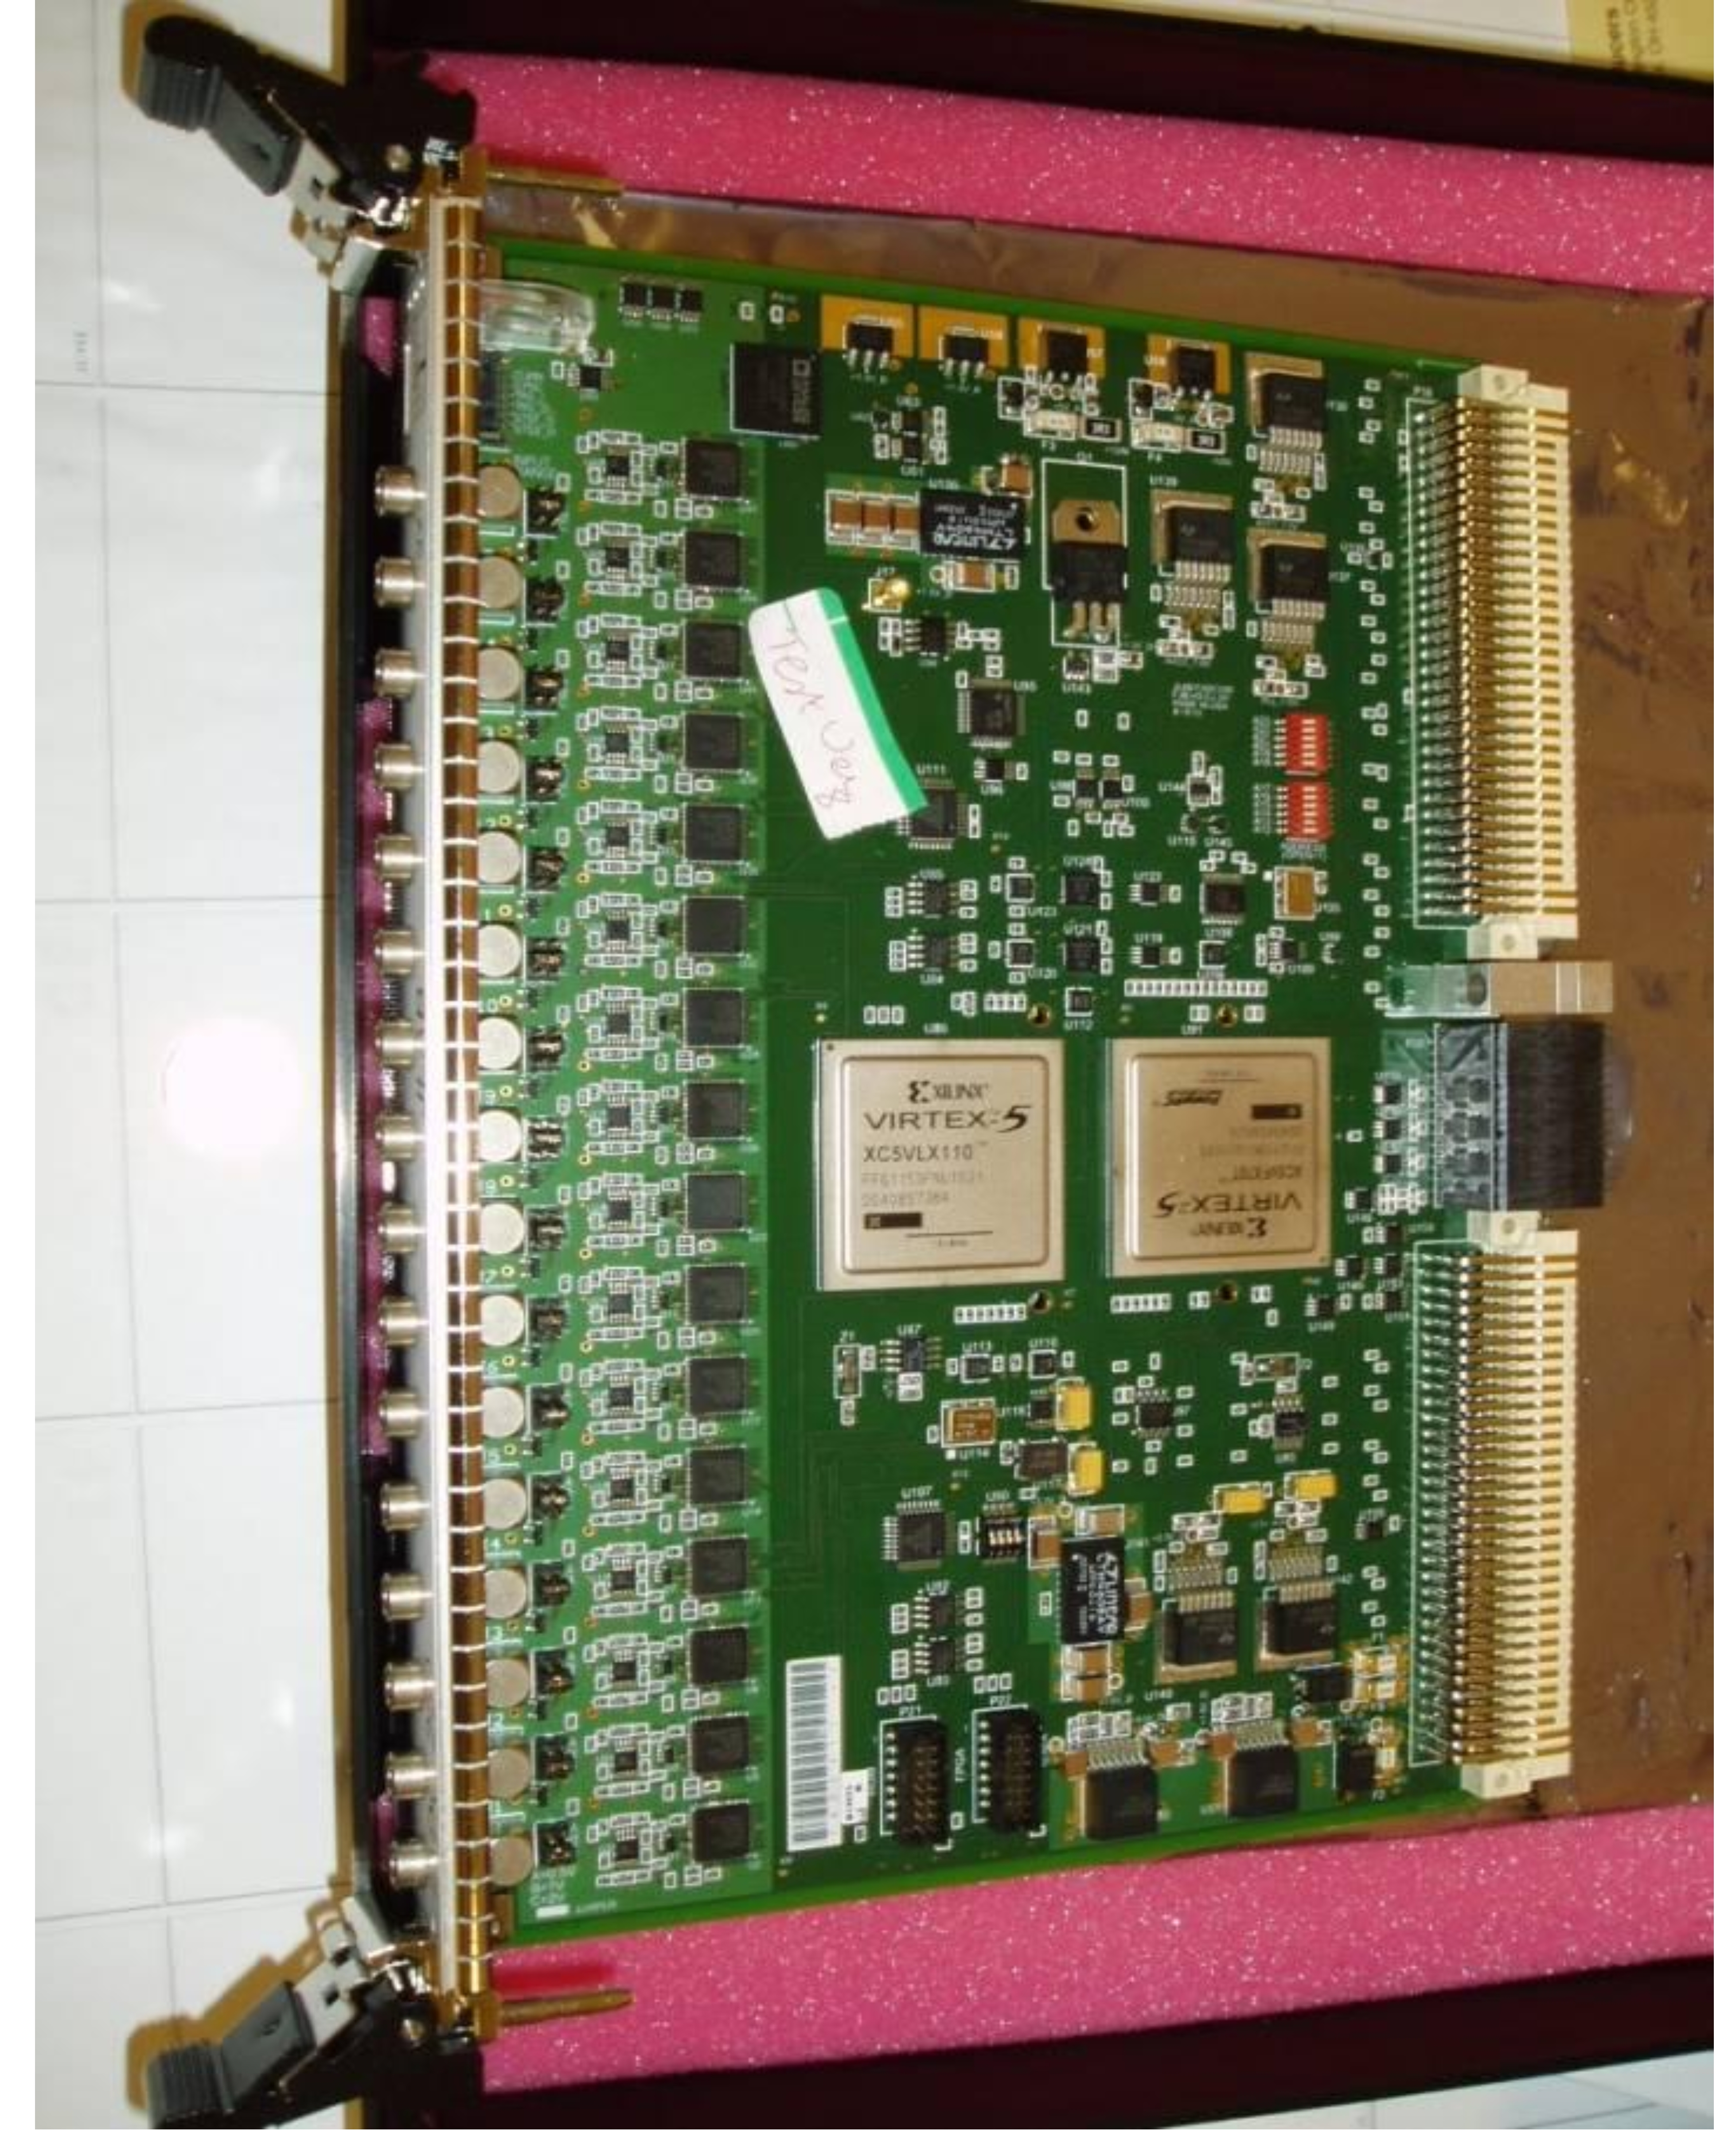
\includegraphics[scale=0.5]{test2012/daq/FADC250_Photo_001.jpg}
\caption{\small{FADC250 VXS module.}}\label{fig:fadc}
\end{figure}

